\chapter{多目的最適化}
\label{chap::multiobjective}

\hspace{1zw}この章では多目的最適化問題の概要と,進化計算による解法について記述する.

\section{問題定義}
ある目的の達成度を,値の小さい(もしくは大きい)ほうが高いものとして関数化したものを目的関数とよぶ.多目的最適化問題とは複数の目的関数集合$\vec{f}(\vec{x})$を最小化(もしくは最大化)する解$\vec{x}$を求める問題である.多目的最適化問題は,以下の式で表現される.

\begin{align}
     & 目的関数:\mbox{Minimize/Maximize} \quad \vec{f}(\vec{x}) = \{f_1(\vec{x}), f_2(\vec{x}),\cdots,f_m(\vec{x})\} \\
     & 制約条件:\mbox{Subject to} \quad ~~~~~~~~~~~~~ \vec{x} \in X
\end{align}
ここで,$m$は目的の数,$\vec{x}$は設計変数(操作可能な変数,決定変数とも呼ぶ),$f_i(\vec{x}) \quad (i=1, 2,\cdots,m)$は設計変数$\vec{x}$から算出されるある目的の達成度を示す目的関数,$X$は設計変数$\vec{x}$の実行可能領域(操作可能範囲)である.


目的の数$m=1$の場合,単目的最適化問題もしくは単一目的最適化問題と呼ぶ.単一目的最適化問題では,真の最適解は一つに定まる.一方,本研究では,上の式で定式化され,目的関数が複数$m \geq 2$であり,複数の目的の間に1つ以上のトレードオフの関係がある多目的最適化問題を取り扱う.$m=2$目的の最小化の目的関数空間を\figref{fig::theory_moo}に例示する.このような問題では,全ての目的関数を同時に最小化することはできない.そこで,操作可能範囲内でこれ以上全ての目的を同時に改善できない解(=パレート最適解)を解候補として定義する.パレート最適解は1つには定まらず解の集合となる.パレート最適解集合からなる超平面を目的関数空間上で表したものをパレートフロントと呼ぶ.多目的最適化とは,パレートフロントのうち少なくとも1点を求めることである.

また,制約を表す実行可能領域$X$は制約関数集合$\vec{g}(\vec{x}) \leq \vec{0}$で表される.ただし,$\vec{g}(\vec{x})=\{g_1(\vec{x}), g_2(\vec{x}),\cdots,g_p(\vec{x})\}$であり,$p$は制約の数である.$p$個の全ての制約を満たす解は実行可能解,一つでも制約を満たさない解は実行不可能解と呼ばれる.

\begin{figure}[ht]
    \begin{center}
        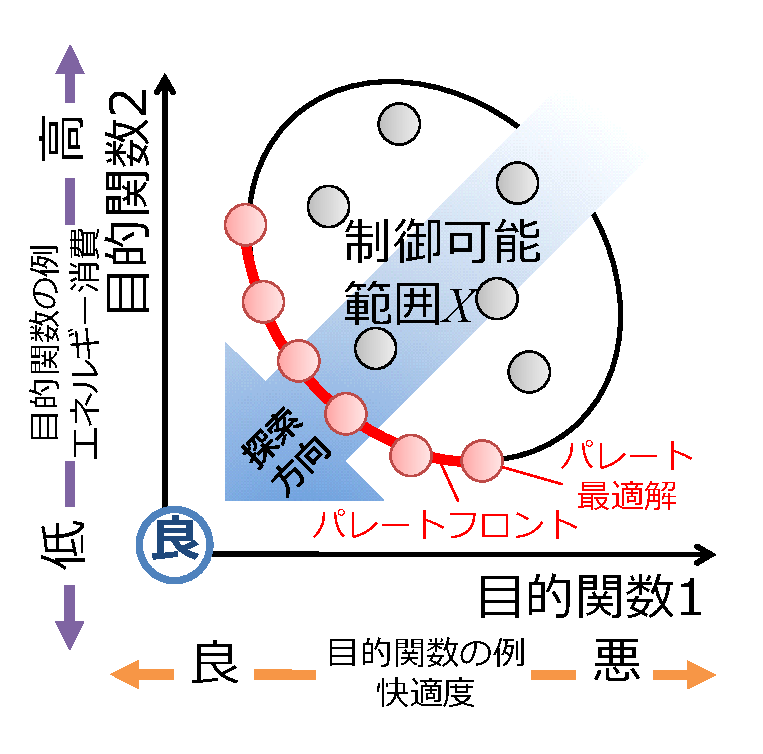
\includegraphics[width=0.6\textwidth,keepaspectratio=true]{fig/theory_moo.eps}
    \end{center}
    \caption{多目的最適化の概念}
    \label{fig::theory_moo}
\end{figure}

多目的最適化問題を解くにあたり重要な概念として,解の優越関係(あるいは支配)がある.2つの解候補を比較したときに,一方が他方に対して全ての目的関数で良い値を持つ場合,その解は他方を優越(dominate, 支配)するという.逆に,全ての目的関数で悪い目的関数値を持つ解は,他方に対し被優越(dominated, 非支配,劣っている)解という.例えば$m=2$目的の最小化問題の\figref{fig::theory_dominate}において2つの解候補$\vec{x}$と$\vec{y}$を比較したときに,$\vec{x}$は$\vec{y}$に対して目的関数1についても目的関数2についても小さい値=良い値であるため,$\vec{x}$は$\vec{y}$を優越することがわかる.また,2つの解候補$\vec{x}$と$\vec{z}$を比較すると,$\vec{x}$は$\vec{z}$に対して,目的関数1については小さい値=良い値だが,目的関数2については大きい値=悪い値であるため,$\vec{x}$は$\vec{z}$を支配しない.また,$\vec{z}$も$\vec{x}$を支配しない.これを非劣もしくは非支配の関係という.\figref{fig::theory_moo}に示すパレート最適解集合は全解集合$X$の非劣解集合であり,多目的最適化では探索中に生成した解集合の中における非劣解集合を獲得することがゴールである.\figref{fig::theory_dominate}に図示する全ての点を生成した解集合だとすると,赤の点が多目的最適化の結果として出力する非劣解集合である.

\begin{figure}[htbp]
    \begin{center}
        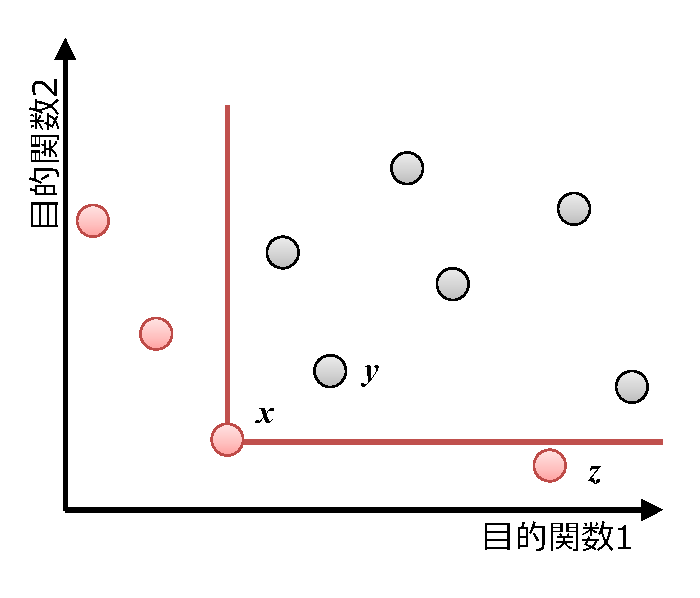
\includegraphics[width=0.6\textwidth,keepaspectratio=true]{fig/theory_dominate.eps}
    \end{center}
    \caption{解の優越関係}
    \label{fig::theory_dominate}
\end{figure}


\section{進化計算による解法}
\subsection{進化計算}\label{subsec::ec}
進化計算(Evolutionary Computation,進化的計算,進化的アルゴリズムとも呼ぶ)とは,生物の進化の過程や群れの動きの様子を模擬する解の集合を利用することによって新たな解を探索する手法の総称である.進化計算の特徴として,以下が挙げられる.
\begin{itemize}
    \item 進化計算はメタヒューリスティクスの一つであり,特定の計算問題に依存しないアルゴリズムである.多様な問題に対して汎用的に対応でき,問題の特性が未知であることがほとんどである実問題に対しても,問題をブラックボックスとして扱って最適化できる.
    \item 解集合を用いて探索する多点探索手法である.多目的最適化では,上述のように最終的にパレートフロントを近似するパレート解集合を求める必要がある.解集合を用いて探索する進化計算は,多目的最適化におけるパレート最適解集合を一回の探索で求めることができ,目的間のトレードオフ関係を考慮した解の意思決定を支援できる.
    \item 確率的に探索する手法である.数理最適化法では問題の厳密解を求めることができるが,進化計算では確率的な探索であるため厳密解を発見する保証はない.厳密解に近い近似解を求めることになる.
\end{itemize}
最も代表的な進化計算は,遺伝的アルゴリズム(GA, Genetic Algorithms)である.GAは生物の進化の過程を模擬したアルゴリズムである.GAは解の候補を生物の個体に見立てて,個体の交叉,淘汰,突然変異による世代交代を模擬する計算を行うことで良好な解を探索する.また,同様に代表的な進化計算として粒子群最適化(PSO, Particle Swarm Optimization)がある.PSOは解集合を魚や鳥などの群れになぞらえ,各個体を群れ全体で方向性をもたせて飛翔させることによって解探索する.この他にも焼きなまし法(SA, Simulated Annealing), 差分進化(DE, Differential Evolution),蟻コロニー最適化(ACO, Ant Colony Optimization), カッコー探索(CS, Cuckoo Search)など様々な手法が提案されている.

進化計算には様々な手法があるが,どの手法も概ね\figref{fig::theory_flow}に示すフローで探索する.ここでは進化計算の探索フローにおける各項目を説明する.

\begin{figure}[ht]
    \begin{center}
        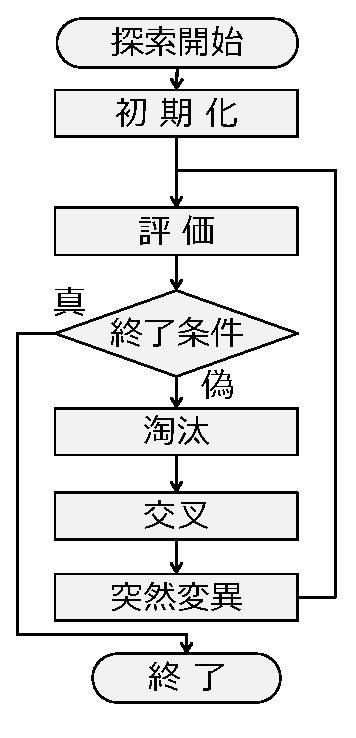
\includegraphics[width=0.3\textwidth,keepaspectratio=true]{fig/theory_flow.eps}
    \end{center}
    \caption{一般的な進化計算アルゴリズムのフロー}
    \label{fig::theory_flow}
\end{figure}

\subsubsection{初期化}
探索に用いる初期解集合を生成する.通常は解の変数それぞれを取りうる範囲の中で一様乱数を用いて決定する.一方で,実問題では通常使用する値やデフォルトの設定値などが存在するため,それを変数とした複数の初期解を用いることもある.また,進化計算では解を個体,解集合を個体群と呼ぶことがある.

\subsubsection{評価}
個体群に含まれる各個体の変数値を使って目的関数値を計算し,個体の評価を行う.


\subsubsection{淘汰}
個体群の中から,次世代に残す個体を選択することを淘汰(または選択)と呼ぶ.淘汰を行う方法にはいくつかの種類があるが,基本的には目的関数値の値の良い解を優先的に次世代に残す方策をとる.進化計算では,選択された解を親(または親個体)と呼ぶことがある.多目的最適化の場合は目的関数が複数あるため,上述の優越関係を用いて淘汰する.最も一般的に用いられる淘汰の方法として,非支配ソートと呼ばれる方法\cite{Deb02}がある.非支配ソートでは,解集合を支配されないレベルでランク分けし,ランクの上位から順序付けする手法である.\figref{fig::theory_rank}に非支配ソートの概念図を示す.解集合のうちどの解にも支配されていない解(非劣解)をランク1として解集合から取り出す.残った解集合の中から,同様に非劣解を取り出してランク2とする.解集合から解がなくなるまでこれを繰り返す.このように解集合をランクで分類し,ランクの値が小さいものほどよい解であると判定して次世代に残す.

\begin{figure}[ht]
    \begin{center}
        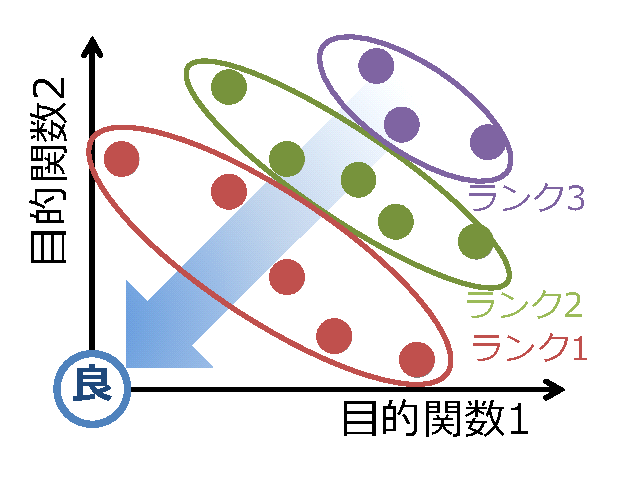
\includegraphics[width=0.6\textwidth,keepaspectratio=true]{fig/theory_rank.eps}
    \end{center}
    \caption{被支配ソートの概念図}
    \label{fig::theory_rank}
\end{figure}

\subsubsection{交叉}
個体群から親個体を選択し,親個体の設計変数の情報をかけ合わせて新たな解を生成する操作を交叉(Crossover)と呼ぶ.進化計算では,交叉によって生成される解を子(または子個体)と呼ぶことがある.交叉方法にも設計変数の種類などによって様々な種類が存在する.ここでは主にGAで用いられる実数値変数用の交叉方法として単峰性正規分布交叉(Unimodal Normal Distribution Crossover, UNDX)\cite{Kita99, Ono97}, Simulated Binary Crossover(SBX)\cite{Agrawal95},さらに粒子群最適化(Particle Swarm Optimization, PSO)\cite{Kennedy95}で用いられる交叉について説明する.
\begin{itemize}
    \item UNDX\cite{Kita99, Ono97}\\
          UNDXは親個体を3つ選択し,親個体集合の重心から正規分布で子を生成する手法である.UNDXによる解の生成方法を\figref{fig::theory_undx}に例示する.UNDXは,親個体群から3つ($\vec{x}_0, \vec{x}_1, \vec{x}_2$)の個体を選択した後,子個体$x_c$を以下の式に従って生成する.
          \begin{align}
              \vec{x}^{c} & = \vec{x}_p + \xi \vec{d}_{01}+D \sum_{i=1}^{n-1} \eta_i \vec{e}_i
          \end{align}
          ここで,$\vec{x}_p$は$\vec{x}_0$と$\vec{x}_1$の中間点$\vec{x}_p = (\vec{x}_0+\vec{x}_1)/2$, $\vec{d}_{01}=\vec{x}_0-\vec{x}_1$, $\xi$は$N(0, \sigma_\xi)$に従う乱数,$\eta_i$は$N(0, \sigma_\eta)$に従う乱数,$D$は$\vec{x}_p$から$\vec{x}_2$へのベクトルの大きさ$|\vec{d}_v| = |\vec{x}_2-\vec{x}_p|$, $\vec{e}_i$は$\vec{d}_{01}$に直交する正規直交基底$\vec{d}_{v}$の基底ベクトルである.
          この式により, 親個体$\vec{x}_0, \vec{x}_1$の中間点を中心として,$\vec{x}_0, \vec{x}_1$方向,$\vec{x}_2$方向それぞれに広がる範囲に乱数で子個体を生成する.
          \begin{figure}[ht]
              \begin{center}
                  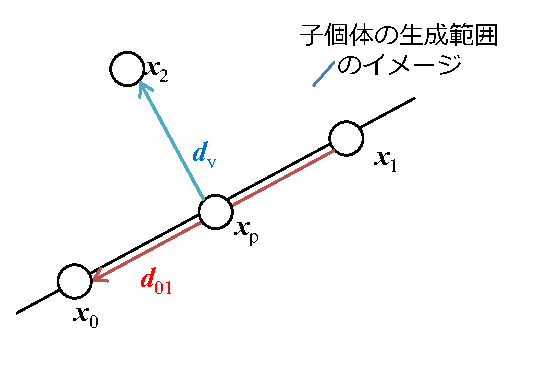
\includegraphics[width=0.5\textwidth,keepaspectratio=true]{fig/theory_undx.eps}
              \end{center}
              \caption{UNDXによる交叉}
              \label{fig::theory_undx}
          \end{figure}

    \item SBX\cite{Agrawal95}\\
          SBXは,親個体2つを選択し,交叉率(Crossover Probability, $P_c$)および分布度(Distribution Index, $\eta_c$)の2つのパラメータにより,確率的に親個体の周囲に新たな解を生成する手法である.SBXは個体の持つ各変数について,1/2の確率で同じ値とし,1/2の確率で次式で算出される値となる.
          \begin{align}
              \beta_i  & =
              \begin{cases}
                  (2u_i)^{\frac{1}{\eta_c+1}} ~~~~~~~~ \mbox{if} \quad u_{i} \leq 0.5, \\
                  (\frac{1}{2(1-u_i)})^{\frac{-1}{\eta_c+1}} \quad \mbox{otherwise},
              \end{cases}                                  \\
              x_i^{a'} & = 0.5 \{(1+\beta_i)x_i^a + (1-\beta_i)x_i^b \}, \\
              x_i^{b'} & = 0.5 \{(1-\beta_i)x_i^a + (1+\beta_i)x_i^b \}.
          \end{align}
          ここで,$x_i^a$, $x_i^b$は選択した2つの親個体$\vec{x}^a$, $\vec{x}^b$の$i$番目の変数,$x_i^{a'}$, $x_i^{b'}$は生成された子個体の$i$番目の変数,$\beta_i$は$i$番目の変数に対する拡散係数,$u_{i}$は$[0,1)$のランダムな値を表す.SBXは,最初に分布度$\eta_c$に基づいて拡散係数$\beta_i$を算出する.また1/2の確率で拡散係数$\beta_i$の符号を反転する.その拡散係数をもとに2つの親個体$\vec{x}^a$, $\vec{x}^b$から子個体の変数を算出する.分布度$\eta_c$は小さいほど周辺の広い範囲に解を生成し,値が大きいほどもとの設計変数近くに解が生成される.

    \item PSO\cite{Kennedy95}\\
          PSOによる交叉を\figref{fig::theory_pso}に例示する.PSOでは,解を粒子に見立て,変数を粒子の現在位置とする.粒子の速度と,個体群(粒子群)のうち良好な粒子方向へのベクトルを\Eqref{eq::theory_pso_velocity}および\Eqref{eq::theory_pso_position}の式により足し合わせることで,次世代の粒子の位置(=変数)を生成する.PSOではこの操作を交叉の代わりに飛翔と呼ぶ.
          \begin{align}
              \vec{v}^{g+1} & = w\cdot \vec{v}^g + c_1 \cdot r_1 (\vec{x}_{pbest}-\vec{x}^g) + c_2 \cdot r_2 (\vec{x}_{gbest} - \vec{x}^g)
              \label{eq::theory_pso_velocity}
              \\
              \vec{x}^{g+1} & = \vec{x}^g + \vec{v}^{g+1}
              \label{eq::theory_pso_position}
          \end{align}
          ここで,$\vec{x}^g$と$\vec{v}^g$は,世代$g$の設計変数空間における粒子の位置と速度である.また,$w$,$c_1$,$c_2$は任意の重み係数,$r_1$と$r_2$は$[0, 1)$の一様乱数である.$\vec{x}_{pbest}$はパーソナルベストの位置で,$\vec{x}_{gbest}$はグローバルベストの位置である.パーソナルベストとは,ある粒子$\vec{x}^g$がこれまで飛翔してきた中で最も目的関数の評価値の高い粒子である.また,グローバルベストとは,ある世代$g$の粒子群の中で最も評価値の高い粒子である.
          \begin{figure}[ht]
              \begin{center}
                  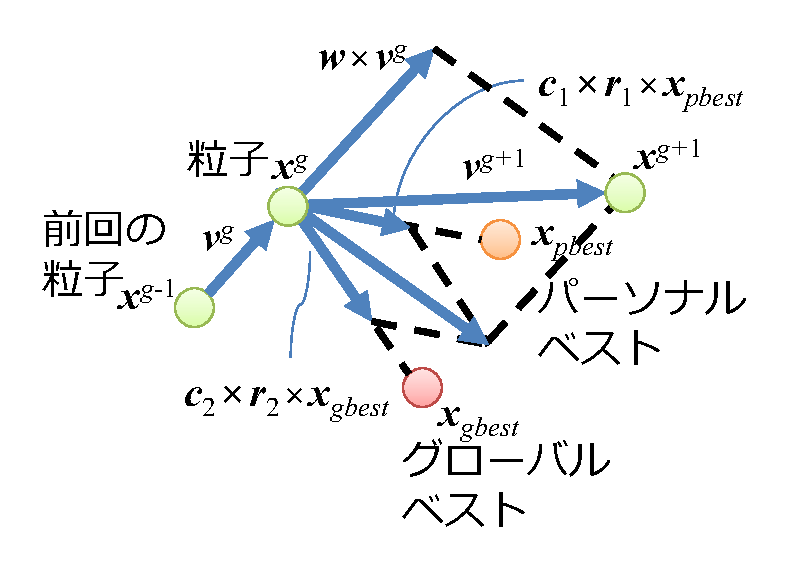
\includegraphics[width=0.5\textwidth,keepaspectratio=true]{fig/theory_pso.eps}
              \end{center}
              \caption{PSOによる交叉}
              \label{fig::theory_pso}
          \end{figure}

\end{itemize}

交叉によって生成された解の変数が変数の取りうる範囲[$x^{min}, x^{max}$]を超過した場合,その解は実行不可能解となってしまうため,超過した変数については実行可能とするよう,境界値まで引き戻す操作を加えることがある.

\subsubsection{突然変異}
交叉によって生成した子個体群の一部の設計変数に対してランダムに操作を加えることを突然変異(Mutation)とよぶ.突然変異には一様突然変異,非一様突然変異などの種類がある.また,設計変数が2値か実数値かによってもいくつか種類がある.ここでは,一般的な一様突然変異,後述のOMOPSOで採用される非一様突然変異,実数値を用いた進化計算アルゴリズムでよく用いられるPolynomial Mutation(PM)について説明する.

\begin{itemize}
    \item 一様突然変異\\
          一様突然変異では,設計変数値ごとに突然変異確率$p_m$で一様乱数値を加える,もしくは一様乱数値に置き換える操作を行う.一様乱数の範囲は,設計変数の取りうる範囲全体$[x^{min}, x^{max}]$や,範囲の1/4を上下に加える$[-0.25(x^{max}- x^{min}), 0.25(x^{max}- x^{min})]$など,いくつかのパターンがある.

    \item 非一様突然変異\cite{Esquivel03}\\
          非一様突然変異では,世代数$g$によって設計変数空間における変異域を変更する.OMOPSOの例では,設計変数値ごとに突然変異確率$p_m$で,次式により新たな$\vec{x}'^{g+1}$を得る非一様突然変異が用いられる.
          \begin{align}
              \small
              x'^{g+1}_i & =
              \begin{cases}
                  x^{g+1}_i+\Delta(g, x^{max}-x^{g+1}_i), \text{if } r_3 < 0.5 & \\
                  x^{g+1}_i-\Delta(g, x^{g+1}_i-x^{min}), \text{otherwise}     & \\
              \end{cases}
              \label{eq::theory_mutation_nonuni}
          \end{align}
          ただし,$\Delta(g, y)$は変異量であり次式で算出する.
          \begin{align}
              \Delta(g, y) = y\cdot\left(1-r^{\left(1-\frac{g}{g_{max}}\right)^b}_4\right)
          \end{align}
          ここで,$x^{g+1}_i$は粒子$\vec{x}^{g+1}$の$i$番目の設計変数の要素,$g_{max}$は総世代数,$r_3$と$r_4$は$[0, 1)$の一様乱数,$b$は変異量を変化させるパラメータである.

    \item PM\cite{Deb96}\\
          PMは突然変異確率(Mutation Probability, $P_m$)と分布度(Distribution Index, $\eta_m$)の2つのパラメータにより突然変異範囲と数を制御する,実数値変数用の突然変異法である.また,世代数によって突然変異確率が変わらない一様突然変異の手法の一つである.突然変異確率$P_m$は解の変数$x_i$に対して,突然変異を適用する確率である.PMによる突然変異後の変数は以下の式で算出する.
          \begin{align}
              \delta_i & =
              \begin{cases}
                  ((2u_{i3}+(1-2u_{i3})(1-\frac{x_i-x_i^{lower}}{\Delta_{i,max}}))^{\eta_m+1})^{\frac{1}{\eta_m+1}-1}          & if \quad u_{i3} \leq 0.5, \\
                  (1-(2(1-u_{i3})+2(u_{i3}-0.5)(1-\frac{x_i^{upper}-x_i}{\Delta_{i,max}}))^{\eta_m+1})^{\frac{1}{(\eta_m+1)}}) & otherwise,                \\
              \end{cases}
              \label{eq::theory_mutation_pm}
          \end{align}
          \begin{align}
              \Delta_{i,max} = x_i^{upper}-x_i^{lower} \\
              x_{i}' = x_{i}' + \delta_i \Delta_{i,max}
          \end{align}
          ここで,$\Delta_{i,max}$は$i$番目の変数の範囲の大きさ,$\delta_i$は$i$次元目の変異係数,$u_{i3}$は$[0,1)$の一様乱数を示す.変異係数$\delta_i$は変数の現在の値と上下限値を考慮して変数の取りうる範囲を超過しないように決定される.

\end{itemize}

PMは変数の取りうる範囲を超過しないよう変異量が決定されるが,一様突然変異や非一様突然変異では変数の取りうる範囲を超過する場合がある.その場合は交叉と同様に超過した変数を境界値まで引き戻す操作を加えることがある.

\subsubsection{終了条件}
進化計算の上述のサイクルを終える条件を定める.最も単純な終了条件は世代や目的関数の評価回数の最大値を定めておき,最大値を超過したら探索を終える,という条件である.その他にも,解集合内の目的関数値が一定以上となった場合や,一定世代改善されなかった場合などに終了する手段がある.

\subsection{NSGA-II\cite{Deb02}}\label{subsec::NSGAII}
NSGA-II(Fast Elitist Non-dominated Sorting Genetic Algorithm)は,GAを用いて多目的最適化問題を解くことができるような工夫を加えた手法であり,多目的進化型アルゴリズムの中でも特に代表的なアルゴリズムである.NSGA-IIのアルゴリズムの流れを以下の\figref{fig::theory_nsga2}に示す.
\begin{figure}[ht]
    \begin{center}
        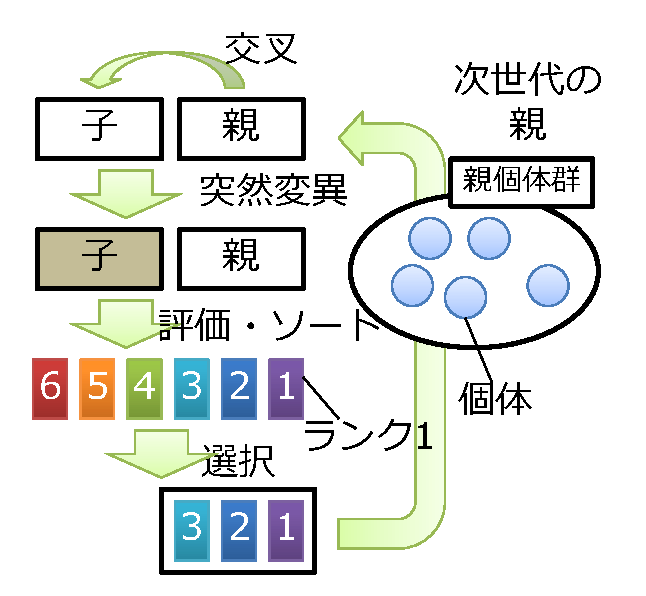
\includegraphics[width=0.6\textwidth,keepaspectratio=true]{fig/theory_nsga2.eps}
    \end{center}
    \caption{NSGA-IIのアルゴリズムのフロー}
    \label{fig::theory_nsga2}
\end{figure}
NSGA-IIは,特に選択(淘汰)において特徴的な操作を行う.NSGA-IIは各世代の解集合を非支配ソートを用いてランキングする.ランク値の良いものから順に次世代の親個体群とする.同一ランクの中で順位付けを行う場合,後述の混雑度の値が大きい順に選択する.混雑度は値が大きいほど周囲に解が存在しないことを示すため,疎な領域から順に解を選択することになる.このようにして得られた親個体群から,交叉によって親個体群と同数の子個体群を生成し同様に淘汰を繰り返すことで,解の進化を行う.

\subsubsection{混雑度}
混雑度(CD: Crowding Distance)は,目的関数空間における解の分布の密集度を表す指標である.混雑度の概念を以下の\figref{fig::theory_crowding_distance}に示す.混雑度は,同一のランク内である解集合をある一つの目的関数値順にソートし,両隣の解の目的関数の差を足し合わせた値である.\figref{fig::theory_crowding_distance}における解$\vec{x}$の混雑距離は$d_{x1}+d_{x2}$となる.また,両端の解は隣接する解が1つしか無いため,混雑距離は$\infty$となる.

\begin{figure}[ht]
    \begin{center}
        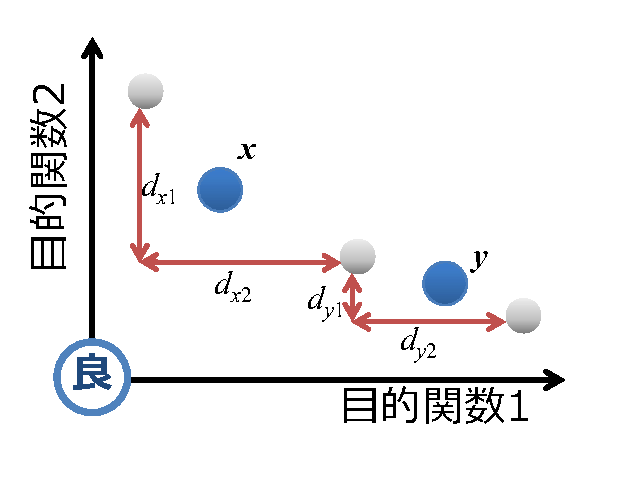
\includegraphics[width=0.5\textwidth,keepaspectratio=true]{fig/theory_crowding_distance.eps}
    \end{center}
    \caption{混雑度の概念図}
    \label{fig::theory_crowding_distance}
\end{figure}

\subsection{OMOPSO\cite{Sierra05}}\label{subsec::OMOPSO}
PSOを用いた多目的最適化手法にMOPSO(Multi-objective Particle Swarm Optimization)がある.OMOPSOは,通常のMOPSOに加え,リーダー粒子群と$\epsilon$-アーカイブという2つの解集合のアーカイブと突然変異操作を導入することにより多目的最適化における探索性能の改善を図ったアルゴリズムである.OMOPSOのアルゴリズムの流れを\figref{fig::theory_omopso}に示す.OMOPSOは,NSGA-IIと同様に解集合(=粒子群)$\mathcal{P}$を非支配ソートと混雑距離でランキングしリーダー粒子群$\mathcal{L}$を抽出する.リーダーを用いて粒子群を飛翔する.その後,粒子群を$\mathcal{Q}, \mathcal{R}, \mathcal{S}$に3分割し,粒子群$\mathcal{Q}$には一様突然変異,粒子群$\mathcal{R}$には非一様突然変異操作を加え,粒子群$\mathcal{S}$には何もしない.粒子群$\mathcal{Q}, \mathcal{R}, \mathcal{S}$を結合して次世代の粒子群$\mathcal{P}$とする.リーダー粒子群と$\epsilon$-アーカイブの和集合$\mathcal{L} \cup \mathcal{E}$の中で$\epsilon$優越する非劣解を$\epsilon$-アーカイブに格納し,最終世代の$\epsilon$-アーカイブ$\mathcal{E}$を非劣解集合として出力する.
OMOPSOの淘汰の手法は,NSGA-IIのように個体群(粒子群)の中から劣解を削除するような手法ではなく,リーダー粒子群と$\epsilon$-アーカイブという2つのアーカイブに良好な解を抽出する手法であるため,必ずしも探索個体群の中に良好な解が残っているとは限らず劣解や制約違反の解が残り続ける場合がある.OMOPSOでは,劣解も含む探索粒子群とリーダー粒子による飛翔をもとに新たな解を探索することと,アーカイブにはこれまでの探索で獲得したすべての$\epsilon$優越する非劣解を格納することで合理的な解を多数獲得できることが特徴である.
\begin{figure}[ht]
    \begin{center}
        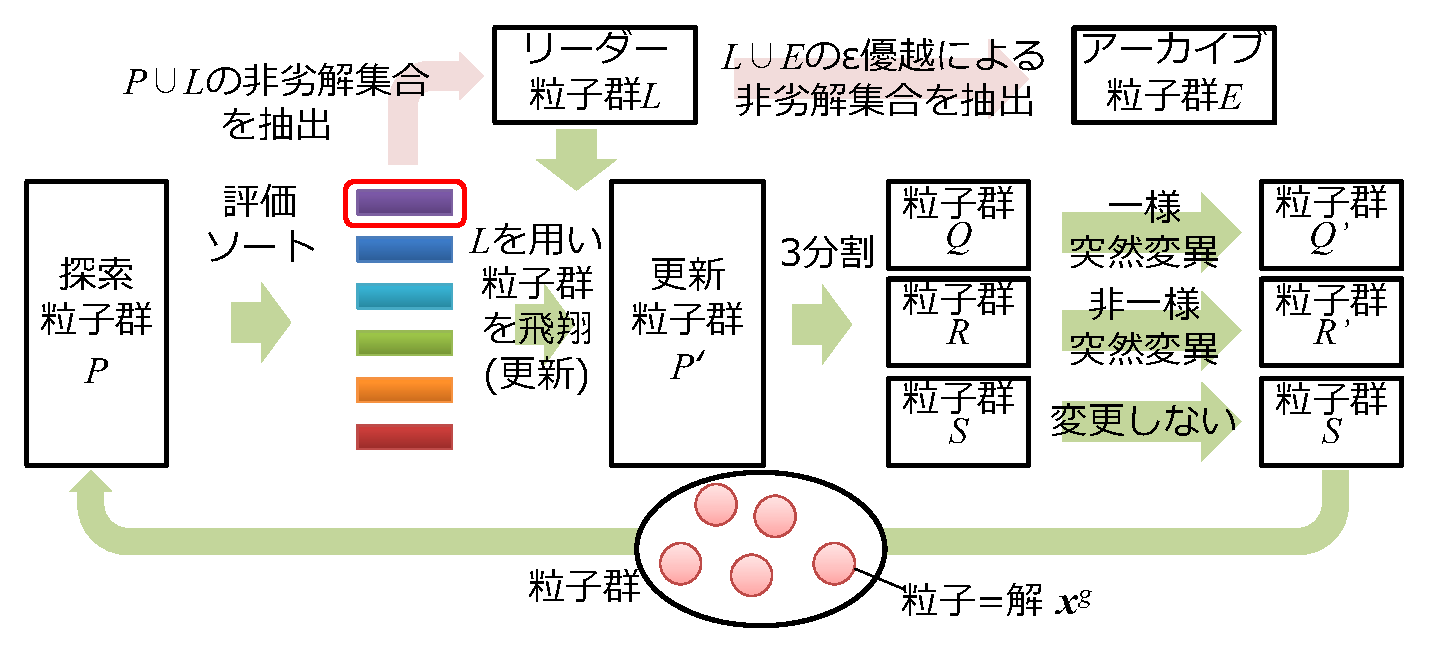
\includegraphics[width=1.0\textwidth,keepaspectratio=true]{fig/theory_omopso.eps}
    \end{center}
    \caption{OMOPSOのアルゴリズムのフロー}
    \label{fig::theory_omopso}
\end{figure}

\subsubsection{$\epsilon$-アーカイブ}
OMOPSOでは$\epsilon$-アーカイブと呼ばれる解集合のアーカイブを持つ.このアーカイブは,探索した解集合のうち,$\epsilon$優越するランク1の解を全て格納する,サイズ制限のないアーカイブである.$\epsilon$優越($\epsilon$-dominance)とは,通常の優越操作に対し,$\epsilon$だけ優越判定範囲を拡大したものである.$\epsilon$-アーカイブによる優越範囲と通常の優越範囲の例を\figref{fig::theory_epsilon_dominance}に示す.\figref{fig::theory_epsilon_dominance}の例では,解$\vec{x}$に対して$\vec{y}$は本来は優越されない位置にいるが,$\epsilon$優越の範囲には含まれるため,この解$\vec{y}$は$\vec{x}$に$\epsilon$優越される,と言う.このように優越範囲を拡張することで,あまりに近傍にある解や,ある1つの目的で大きく劣っている解を削除した合理的な解集合をアーカイブに残すことができる.

\begin{figure}[ht]
    \begin{center}
        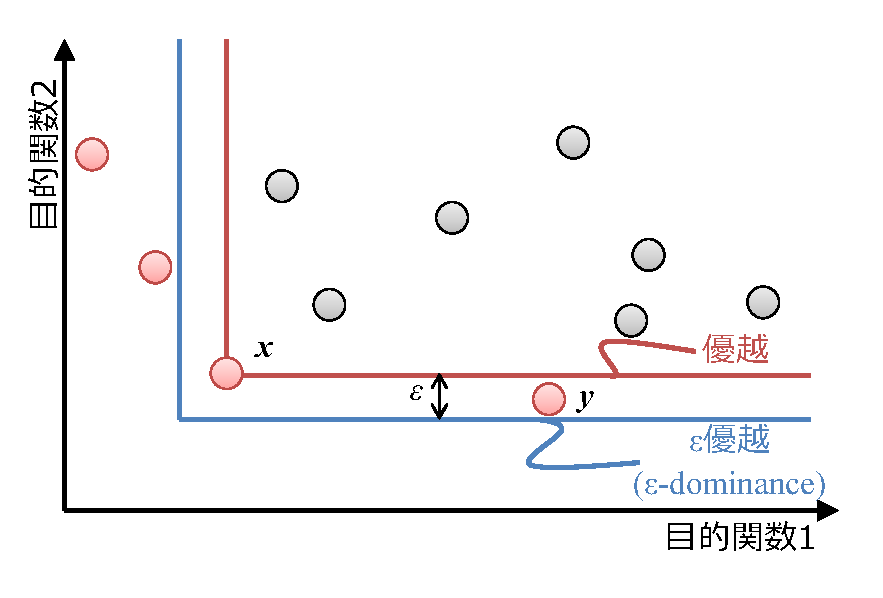
\includegraphics[width=0.7\textwidth,keepaspectratio=true]{fig/theory_epsilon_dominance.eps}
    \end{center}
    \caption{$\epsilon$優越の概念図}
    \label{fig::theory_epsilon_dominance}
\end{figure}

\subsubsection{OMOPSOのアルゴリズム}
OMOPSOの具体的なアルゴリズムを以下に示す.
\begin{description} \label{algo::OMOPSO}
    \setlength{\listparindent}{0pt}   %5. 最初のインデント
    \setlength{\itemsep}{0pt}      %2. ブロック間の余白    
    \item[Step 1:] サイズ$N^{\mathcal{P}}$のベース粒子群$\mathcal{P}$をランダムに生成し,世代数$g=0$にする.
    \item[Step 2:] 各粒子$\vec{x}^g \in \mathcal{P}$について,目的関数値と制約関数値を求め,パーソナルベストとする.
    \item[Step 3:] ベース粒子群$\mathcal{P}$における非劣粒子群をリーダー粒子群$\mathcal{L}$とアーカイブ粒子群$\mathcal{E}$にコピーする.
    \item[Step 4:] 各粒子$\vec{x}^g \in \mathcal{P}$の速度と位置を\Eqref{eq::theory_pso_velocity}, \eqref{eq::theory_pso_position}で更新する.ただし,$\vec{x}_{gbest}$は$\mathcal{L}$からバイナリトーナメント選択で選択された粒子の位置とする.更新した$\vec{x}^{g+1}$の各要素が,[$x^{min}, x^{max}$]の範囲を超過した場合,境界値まで引き戻し,さらに速度$\vec{v}^{g+1}$を$-1$倍する修復操作を施す.
    \item[Step 5:] $\mathcal{P}$を粒子群$\mathcal{Q}$,$\mathcal{R}$,$\mathcal{S}$へ均一に分割する.
    \item[Step 6:] 粒子群$\mathcal{R}$の各粒子に$[-0.25(x^{max}- x^{min}), 0.25(x^{max}- x^{min})]$の範囲の一様乱数値を加える一様突然変異,粒子群$\mathcal{S}$の各粒子に\Eqref{eq::theory_mutation_nonuni}による非一様突然変異を施し,粒子群$\mathcal{Q}$には何もしない.
    \item[Step 7:] 粒子群$\mathcal{Q}$, $\mathcal{R}$, $\mathcal{S}$を結合し,新たな粒子群$\mathcal{P}$ (=$\mathcal{Q}\cup\mathcal{R}\cup\mathcal{S}$)とする.
    \item[Step 8:] 粒子群$\mathcal{P}$の各粒子を評価し,目的関数値と制約関数値を求め,パーソナルベストを後述の制約支配する場合,パーソナルベストを更新する.
    \item[Step 9:] $\mathcal{P} \cup \mathcal{L}$の粒子群における非劣粒子群をリーダー粒子群$\mathcal{L}$にする.同様に,$\mathcal{L} \cup \mathcal{E}$の粒子群における非劣粒子群をアーカイブ粒子群$\mathcal{E}$にする.リーダー粒子群$\mathcal{L}$がサイズ$N^{\mathcal{L}}$を超過する場合,混雑距離の上位$N^{\mathcal{L}}$までを$\mathcal{L}$に残し,それ以外は$\mathcal{L}$から削除する.
    \item[Step 10:] 世代数$g$に1を加算し,総世代数$g_{max}$に達したとき,アーカイブ粒子群$\mathcal{E}$を最適化の結果として出力して終了する.そうでなければ{\bf Step 4}に戻る.
\end{description}



\subsection{制約条件の取り扱い\cite{Coello02, Harada07}}
進化計算のように多数の解集合を交叉と世代交代によってパレート最適解集合を探索する手法は,探索過程において実行不可能解を生成することがある.また,実行可能範囲が狭い問題や偏りのある問題では,初期解をランダムに生成しても実行可能解は生成されず,探索初期には実行可能解を探索しなければならない場合がある.そこで,探索中の制約の取り扱い方法がいくつか考案されている.ここでは標準的に用いられる手法と,本研究で採用する制約優越について述べる.

\subsubsection{デス・ペナルティ法}
デス・ペナルティ法(Death Penalty)は,探索中の解集合のうち実行不可能解を削除する方法である.これによって探索によって得られた実行可能解を残し,実行可能解のみから交叉することによって新たな実行可能解の探索を促進する.一方で,上述のように実行可能範囲が狭い問題では,新たに生成される子個体の多くが削除されてしまい,探索が進まないことがある.

\subsubsection{ペナルティ法}
解が制約を満たさない場合に,制約違反の度合い(制約違反量, Constraint Violation Degree)を計算する関数(ペナルティ関数)$v(\vec{x})$を定義し,ペナルティ関数値を目的関数値に足し合わせて,それを最小化(もしくは最大化)することによって,実行可能解と同時に目的関数値の良い解を探索する手法である.ペナルティ法で用いられる制約なし多目的最適化問題は,以下のように定義される.

\begin{align}
    \mbox{Minimize/Maximize} \quad \vec{f}(\vec{x}) + v(\vec{x})
\end{align}

本手法に対しては,ペナルティ関数のレンジを目的関数に合わせて調整するなど適切なペナルティ関数を定義しなければならないこと,目的関数に対応しない制約が複数存在する場合に適用が困難なことが課題として挙げられている.

\subsubsection{制約の目的関数化}
制約違反量を,追加目的関数とした多目的最適化問題を解くことにより,実行可能でかつ目的関数の良好な解を探索する手法である.制約を目的として追加した新たな目的関数は,以下のように定義される.

\begin{align}
    \mbox{Minimize/Maximize} \quad \vec{f}(\vec{x}) = \{f_1(\vec{x}), \cdots,f_m(\vec{x}), g_1(\vec{x}), \cdots, g_p(\vec{x})\}
\end{align}
この手法では,制約条件も目的関数とすることで,制約を満たしながら良好な解を探索できる,ある程度制約違反を許容しつつ目的関数値の良い解も探索できる,という利点がある.そのため,制約が,必ず満たさなければならない強い制約ではなく,ある程度の違反が許容される弱い制約である場合や,制約条件の範囲が未確定である場合に有効である.一方で,本手法をとると問題によっては最終世代の解集合に実行不可能な解が残ってしまうことになる.そのため,最終世代のパレート解集合のうち実行可能解は限定されてしまい,全ての個体を有効に活用できない場合がある.

\subsubsection{制約優越法\cite{Deb02}}
制約優越法は,ペナルティ法と同様にペナルティ関数$v(\vec{x})$を定義する.ある2つの解の優越を比較をする際に,いずれも制約を満たすかどうか,制約を満たす場合は目的関数値で,制約を満たさない場合は制約違反量で優越判定をすることで,制約を満たし,かつ目的関数値が良好である解の探索を促進する手法である.2つの解$\vec{x}$, $\vec{y}$について,$\vec{x}$が$\vec{y}$に制約優越する(または制約支配する)という場合は以下のいずれかを満たすことを指す.

\begin{itemize}
    \item $\vec{x}$が実行可能であり,$\vec{y}$が実行不可能である
    \item $\vec{x}$と$\vec{y}$両方が実行不可能で,$\vec{x}$の制約違反量$v(\vec{x})$が$\vec{y}$の制約違反量$v(\vec{y})$に対して小さい$(v(\vec{x})<v(\vec{y}))$
    \item $\vec{x}$と$\vec{y}$両方が実行可能で,$\vec{x}$の目的関数が$\vec{y}$を優越している
\end{itemize}

制約優越では,ペナルティ法とは異なりペナルティ関数のレンジを目的関数に合わせる必要がないこと,目的関数の数に依存せずペナルティ関数を定義できることから,目的関数に関わらない種々の制約を持つ実問題においても容易に制約を扱うことができる.そこで,本研究では,制約優越を採用することで制約条件を取り扱う.
